% 
%            ,,                                        
%          `7MM            _.o9                                
%            MM                                             
%  ,6"Yb.    MM  ,p6"bo   ,6"Yb.  M"""MMV  ,6"Yb.  `7Mb,od8 
% 8)   MM    MM 6M'  OO  8)   MM  '  AMV  8)   MM    MM' "' 
%  ,pm9MM    MM 8M        ,pm9MM    AMV    ,pm9MM    MM     
% 8M   MM    MM YM.    , 8M   MM   AMV  , 8M   MM    MM     
% `Moo9^Yo..JMML.YMbmd'  `Moo9^Yo.AMMmmmM `Moo9^Yo..JMML.   
% 
% 
% Free and Open-Source template for academic works
% https://github.com/dpmj/alca



\subsection{Accenni di Cloud Computing}

Nel contesto di Kubernetes, il cloud computing offre una serie di vantaggi significativi. Kubernetes, essendo un sistema di orchestrazione di container, può essere efficacemente sfruttato nel contesto di un ambiente cloud per scalare dinamicamente le risorse, gestire il bilanciamento del carico e garantire l'affidabilità delle applicazioni distribuite.

L'utilizzo del cloud computing per Kubernetes consente una distribuzione agnostica del fornitore, dove i cluster Kubernetes possono essere eseguiti su diverse piattaforme cloud o ambienti on-premise. Ciò offre un elevato grado di flessibilità, permettendo agli sviluppatori di adattarsi alle esigenze specifiche dell'applicazione senza essere vincolati a una piattaforma specifica.

Inoltre, il cloud computing facilita l'implementazione di servizi aggiuntivi che possono migliorare ulteriormente l'esperienza di sviluppo e gestione di Kubernetes. Questi possono includere servizi di monitoraggio, sicurezza, gestione delle identità e dei servizi di archiviazione avanzati che possono essere facilmente integrati nell'ecosistema Kubernetes ospitato nel cloud.

Un esempio di approfondimento su come il cloud computing e Kubernetes possono essere sinergici può essere trovato in \cite{armbrust2010view}. Questo studio discute il paradigma del cloud computing e il ruolo di sistemi distribuiti e scalabili nell'elaborazione dei dati su grandi infrastrutture cloud.

Kubeflow, così come le alternative presentate, può giovare ampiamente dal cloud computing. Specifici cloud provider offrono sistemi di Kubernetes-as-a-service che permettono una rapida integrazione di Kubeflow.

\subsubsection{AWS Elastic Kubernetes Service}

\textbf{AWS Elastic Kubernetes Service} (EKS) è un servizio completamente gestito offerto da Amazon Web Services (AWS) che semplifica il processo di esecuzione, gestione e scalabilità di applicazioni basate su container utilizzando Kubernetes. Il servizio mira a offrire un'esperienza utente senza complicazioni, consentendo agli sviluppatori di concentrarsi sulla creazione delle proprie applicazioni senza doversi preoccupare dell'amministrazione complessa e della gestione dell'infrastruttura Kubernetes sottostante.

Con AWS EKS, gli utenti possono creare cluster Kubernetes in modo rapido ed efficiente, beneficiando della scalabilità e della sicurezza garantite dall'infrastruttura di AWS. Il servizio integra nativamente con altri servizi AWS, offrendo un ecosistema completo per la distribuzione di applicazioni containerizzate su larga scala.

EKS semplifica la gestione del ciclo di vita del cluster, fornendo aggiornamenti automatici per le versioni di Kubernetes e gestendo la distribuzione di patch di sicurezza. Questo riduce il carico operativo sugli amministratori di sistema e garantisce che i cluster siano sempre aggiornati e protetti.

\begin{figure}[h]
    \centering
    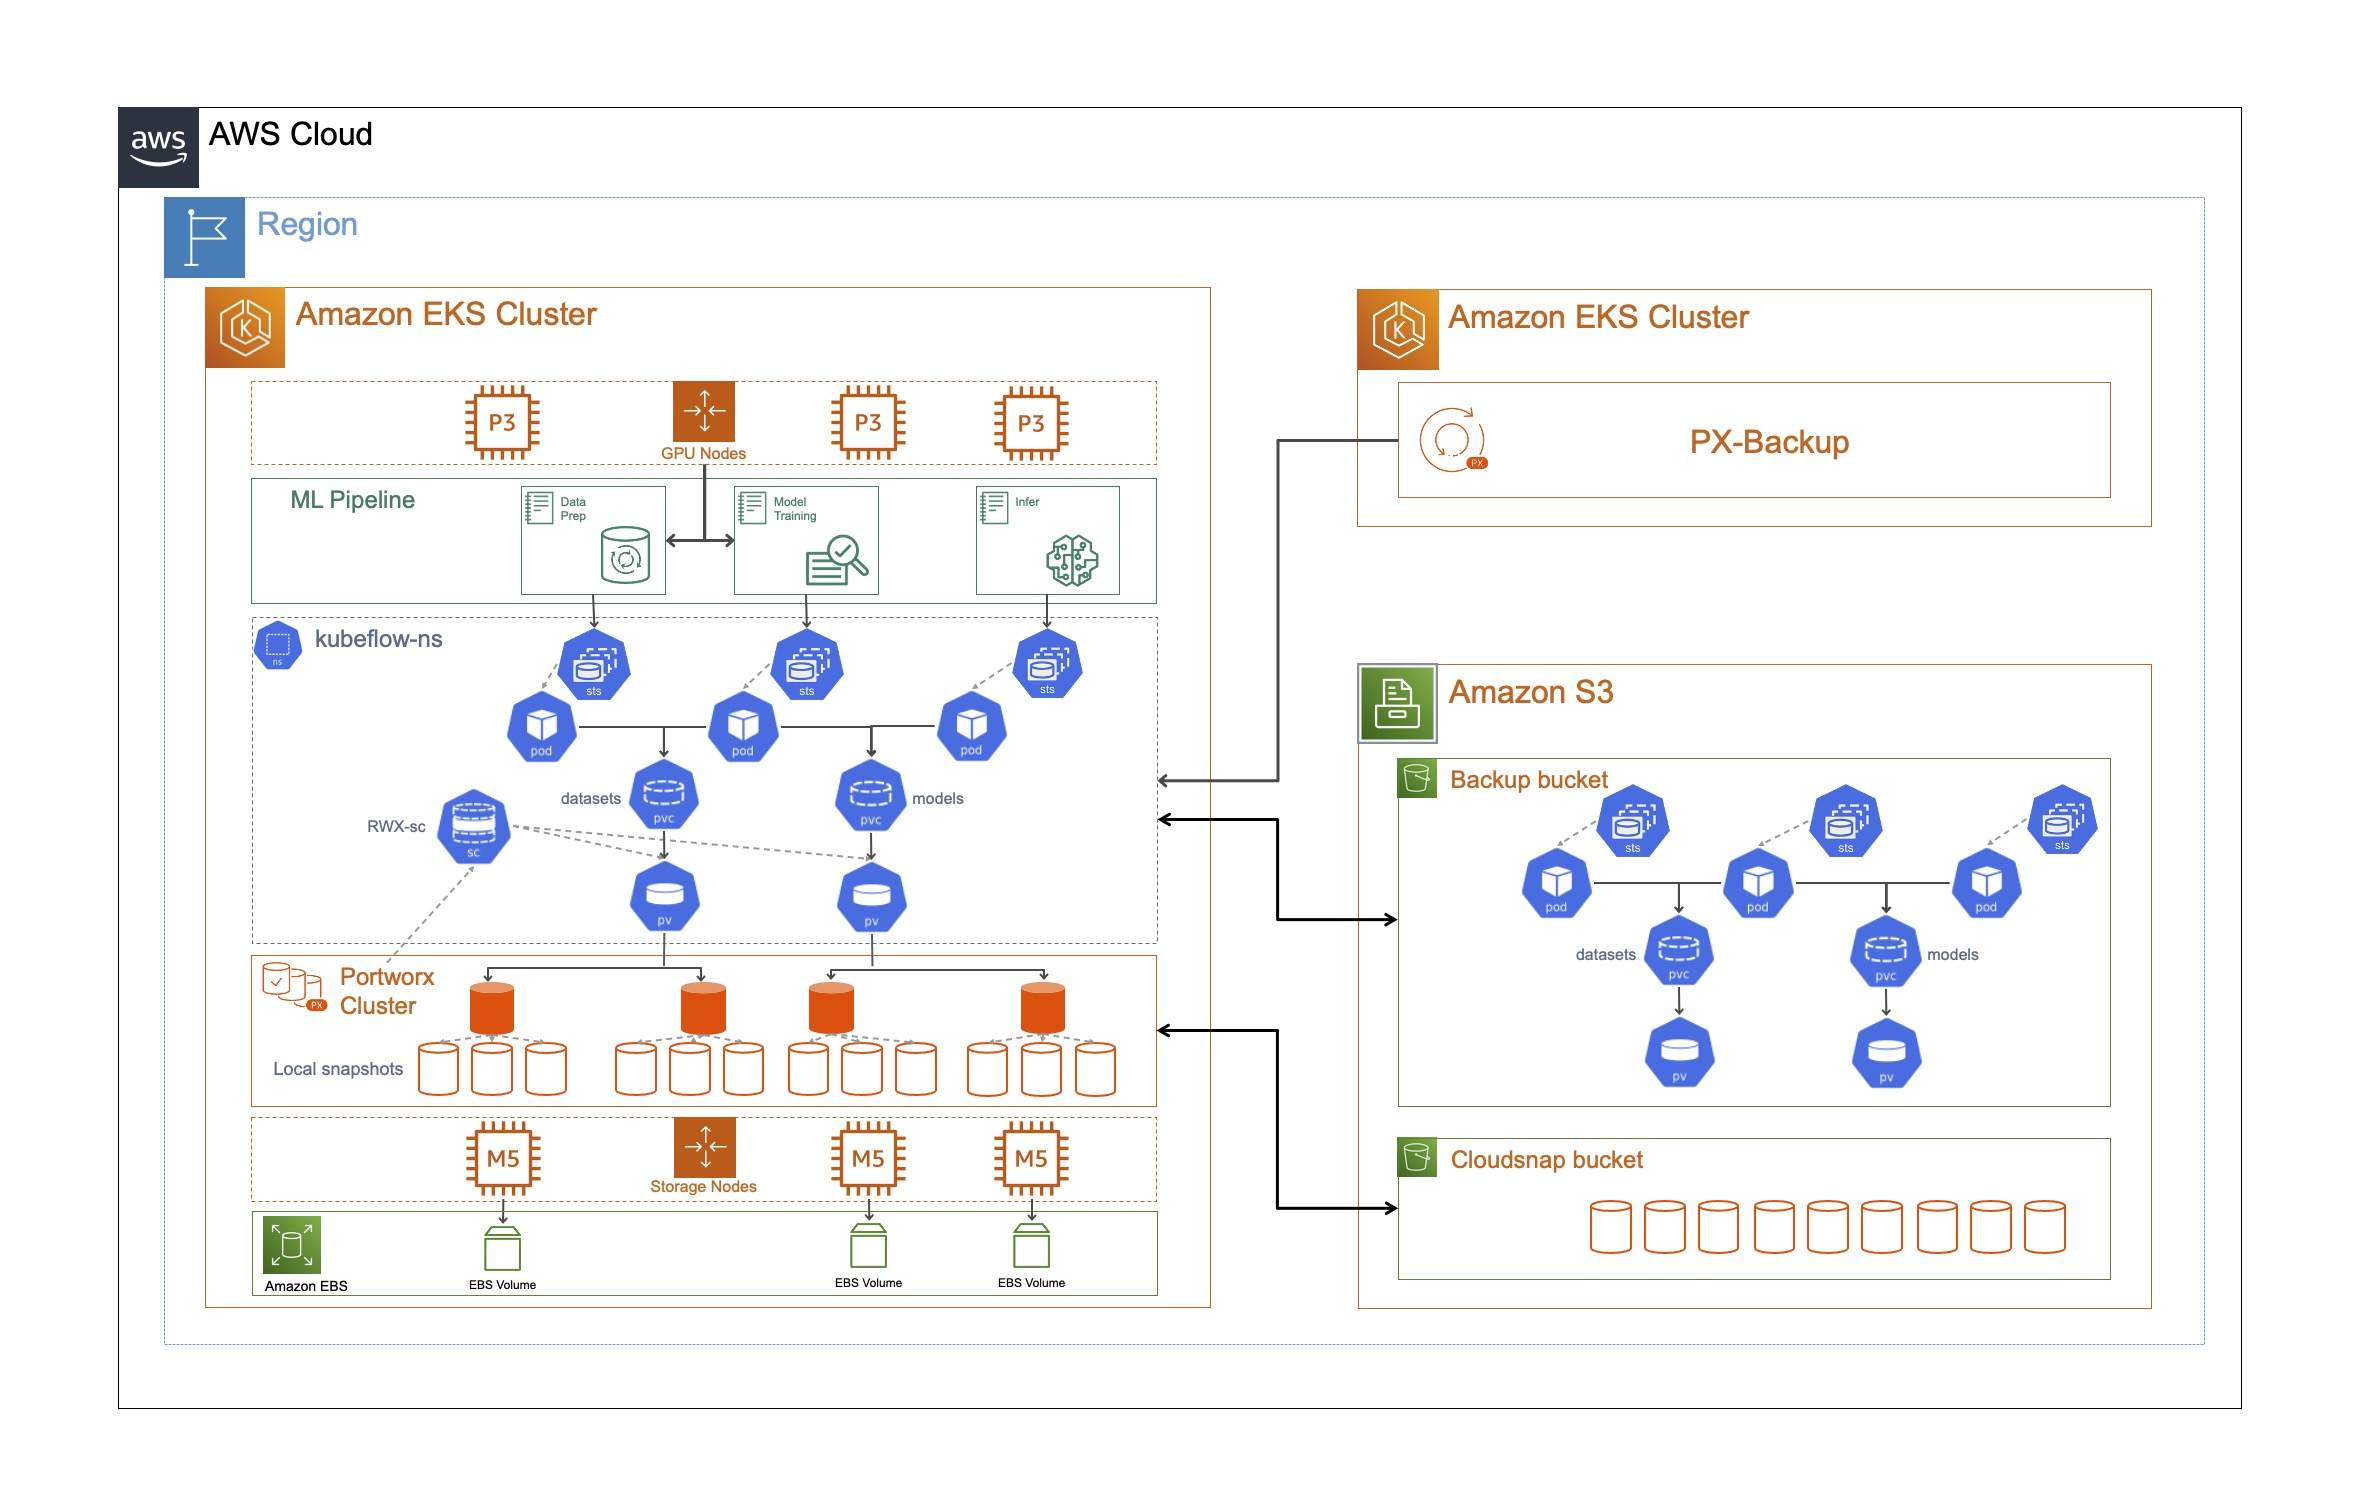
\includegraphics[width=\linewidth]{figures/ch3/kubeflow-aws.jpeg}
    \caption[Kubeflow su AWS Elastic Kubernetes Service]{Kubeflow su AWS Elastic Kubernetes Service}
    \label{fig:cha3:kf-aws}
\end{figure}

Il servizio offre anche integrazioni con strumenti AWS esistenti come Amazon CloudWatch per il monitoraggio e AWS Identity and Access Management (IAM) per il controllo degli accessi e la gestione delle identità. Ciò facilita la creazione di flussi di lavoro integrati e sicuri per le applicazioni Kubernetes su AWS.

Inoltre, EKS è progettato per essere altamente resiliente, garantendo la disponibilità del cluster e la gestione automatica dei nodi. L'elasticità di AWS consente la scalabilità dinamica dei cluster in base ai requisiti del carico di lavoro, garantendo che le applicazioni siano eseguite in modo efficiente e affidabile.

In sintesi, AWS Elastic Kubernetes Service offre un ambiente completamente gestito per eseguire applicazioni containerizzate su Kubernetes su AWS. Integra funzionalità avanzate di AWS per semplificare la gestione, garantire la sicurezza e consentire la scalabilità delle applicazioni containerizzate su una delle principali piattaforme cloud al mondo.

\subsubsection{GCP Google Kubernetes Engine}

\textbf{Google Kubernetes Engine} (GKE) è un servizio completamente gestito offerto da Google Cloud Platform (GCP) per orchestrare e gestire container basati su Kubernetes. GKE semplifica la creazione, la gestione e l'implementazione di applicazioni containerizzate, fornendo un'infrastruttura scalabile e affidabile per eseguire ambienti Kubernetes.

GKE si basa sulla potente piattaforma Kubernetes e offre un'esperienza utente senza problemi. Consente agli sviluppatori di concentrarsi sulla creazione di applicazioni senza la necessità di gestire l'infrastruttura sottostante. GKE supporta Kubernetes nativamente, fornendo agli utenti l'accesso a tutte le funzionalità e le capacità di orchestrazione di Kubernetes, senza doversi preoccupare della complessità della gestione del cluster.

Il servizio GKE è progettato per integrarsi perfettamente con altri servizi GCP, offrendo una soluzione completa per le esigenze di distribuzione di applicazioni containerizzate. Ad esempio, GKE integra nativamente con Google Cloud Identity per garantire il controllo degli accessi e la sicurezza delle risorse.

\begin{figure}[h]
    \centering
    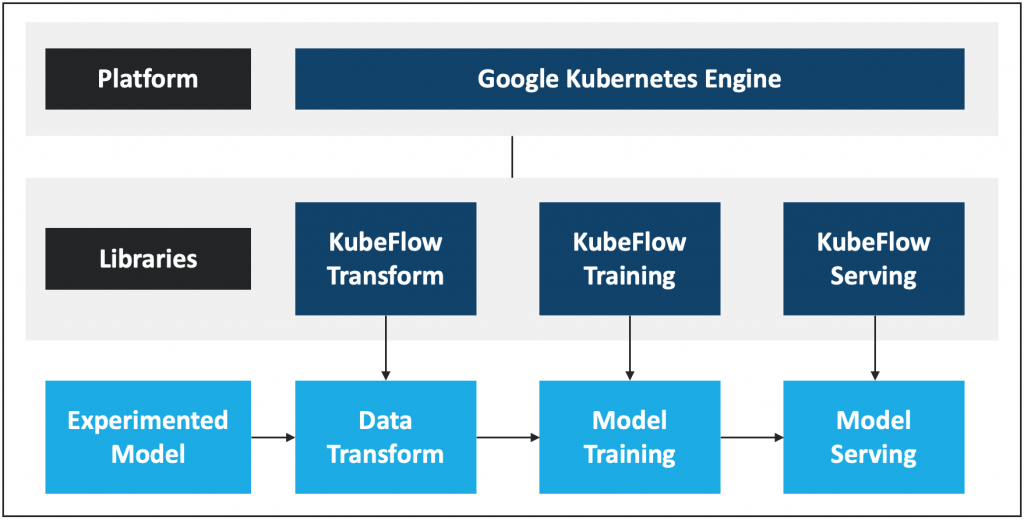
\includegraphics[width=300px]{figures/ch3/kubeflow-gcp.png}
    \caption[Kubeflow su GCP Google Kubernetes Engine]{Kubeflow su GCP Google Kubernetes Engine}
    \label{fig:cha3:kf-gcp}
\end{figure}

GKE offre funzionalità avanzate come il bilanciamento del carico automatico, l'auto-scaling e l'aggiornamento automatico dei nodi. Queste funzionalità semplificano la gestione delle risorse e consentono alle applicazioni di adattarsi dinamicamente ai cambiamenti nei requisiti del carico di lavoro.

Grazie alla rete planetaria di Google Cloud, GKE consente di distribuire cluster Kubernetes in diverse regioni del mondo, garantendo una bassa latenza e una maggiore disponibilità. Ciò è particolarmente utile per applicazioni che richiedono una presenza globale.